\documentclass[a4paper,12pt]{article}
% --- Pacchetti Fondamentali ---
\usepackage[utf8]{inputenc} % Codifica caratteri
\usepackage[T1]{fontenc}    % Codifica font
\usepackage[italian]{babel} % Lingua italiana
\usepackage{geometry}       % Gestione margini
\geometry{a4paper, margin=2.5cm}

% --- Pacchetti Matematica e Fisica ---
\usepackage{amsmath, amssymb} % Simboli matematici
\usepackage{siunitx}          % Gestione unità di misura e numeri (FONDAMENTALE)
\sisetup{
    output-decimal-marker = {.}, % Punto come separatore decimale
    separate-uncertainty = true, % Scrive errori come (Valore +/- Errore)
    per-mode = symbol            % Usa / per le unità (m/s)
}
\usepackage[version=4]{mhchem} % Per scrivere reazioni
\DeclareSIUnit\angstrom{\text{\AA}}

% --- Pacchetti Immagini e Tabelle ---
\usepackage{graphicx} % Per inserire PNG/JPG
\usepackage{float}    % Per forzare la posizione delle immagini (H)
\usepackage{multirow}
\usepackage{booktabs}
\usepackage[justification=centering]{caption}  % Per personalizzare le didascalie
\usepackage{subcaption}

% --- Dati Intestazione ---
\title{\textbf{Titolo dell'Esperienza}}
\author{Filippo Audisio, Cataldo Insalaco, Telemaco Pezzoni}
\date{\today}

\begin{document}

    \maketitle

    % -------------------------------------------------------------------
    \section{Obiettivo dell'esperienza}
        L'obiettivo dell'esperienza è quello di studiare, tramite il software SRIM, la dose ricevuta da alcuni decadimenti di cattura neutronica usati in ambito medico.

    % -------------------------------------------------------------------
    \section{Materiali e Metodi}

        \subsection{Strumentazione utilizzata}
            L'unico strumento utilizzato è il software SRIM per simulare i vari casi studiati.

        \subsection{Procedura sperimentale}
            Si sono studiati 3 casi di cattura neutronica:
            \begin{itemize}
                \item BNCT (Boron Neutron Capture Therapy): 
                    \\ \ce{^{10}B + n -> ^{7}Li + \alpha} (b.r. 6\%)
                    \\ \ce{^{10}B + n -> ^{7}Li + {\alpha} + \gamma} (b.r. 94\%)
                \item LiNCT (Lithium Neutron Capture Therapy): 
                    \\ \ce{^{6}Li + n -> ^{3}H +\alpha}
                \item Nitrogen Neutron Capture: 
                    \\ \ce{^{14}N + n -> ^{14}C + ^{1}H}
            \end{itemize}
            In tutti e tre i casi per calcolare la dose su SRIM si è supposto che la cattura neutronica fosse già avvenuta e si è calcolato solo il contributo dei prodotti di reazione.
            Le cellule sono state modellate come dei cubi di lato 10 \unit{\micro\meter}.
            All'inizio si è supposto che i decadimenti avvenissero sulla superficie esterna della cellula, perfettamente a metà di una faccia del cubo, e si è calcolata la dose ricevuta dalla cellula e da quella limitrofa.
            SRIM permette di simulare un nuclide alla volta e restituisce il range, il profilo della ionizzazione e l'energia depositata in \unit{\electronvolt / (\text{ione} \cdot \angstrom)}.
            Da SRIM quindi possiamo ricavare l'energia depositata nella cellula andando a sommare l'energia depositata in ogni segmento \unit{\angstrom} fino a raggiungere i 10 \unit{\micro\meter} che è la lunghezza della cellula.
            SRIM restituisce anche la densità del tessuto utilizzato, la pelle nel nostro caso, e da questa si può ricavare la massa della cellula.
            Si può quindi calcolare la dose assorbita dalla cellula come $\frac{E_{tot}}{m}$.
            Lo stesso calcolo lo si fa per la cellula limitrofa.
            \\
            Nella seconda parte si è supposto che il decadimento non avvenisse più sulla superficie, ma al centro della cellula.
            Usando lo stesso procedimento del primo punto si è calcolata la dose assorbita dalla cellula e dalla cellula limitrofa.
            \\
            Nell'ultimo punto dell'esperienza abbiamo generato delle coordinate e delle direzioni casuali per le particelle in ogni decadimento.
            Questo perchè, nella realtà, i decadimanti non avvengono tutti nello stesso punto sulla superficie o al centro della cellula, ma avvengono in modo casuale all'interno di questa.
            Anche in questo caso abbiamo calcolato energia, quindi la dose assorbita dalla cellula sorgente e dalla cellula limitrofa.
            
    % -------------------------------------------------------------------
    \section{Dati sperimentali e Analisi}
        \subsection{Grafici simulazione}
            \textbf{Decadimento sulla superficie o al centro della cellula}
            \begin{itemize}
                \item Boro: decadimento con branching ratio 6\%
                \begin{figure}[H]
                    \centering
                    \begin{subfigure}{0.33\textwidth}  
                        \centering
                        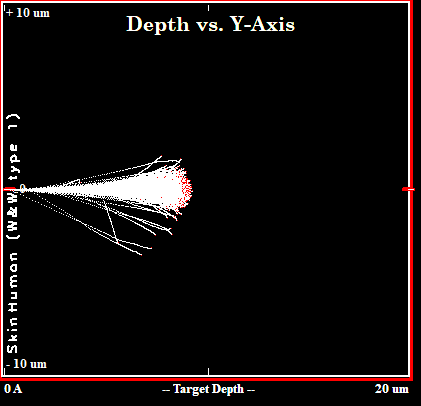
\includegraphics[width=\textwidth]{dati/boro_6/alfa_boro_6/alfa_boro_6.png}
                        \caption{$\alpha$ ($E_{\alpha}$ = 1.78 MeV)}
                        \label{fig:alpha_boro_6}
                    \end{subfigure}\hfill
                    \begin{subfigure}{0.33\textwidth}  
                        \centering
                        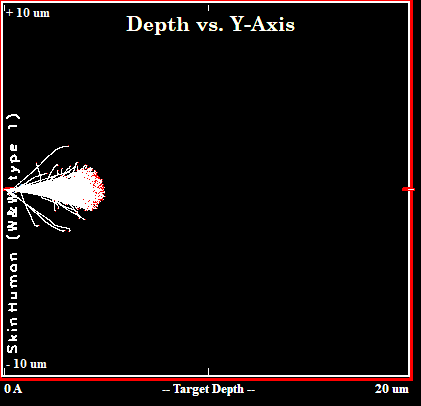
\includegraphics[width=\textwidth]{dati/boro_6/litio_boro_6/litio_boro_6.png}
                        \caption{Litio ($E_{Li}$ = 1.01 MeV)}
                        \label{fig:litio_boro_6}
                    \end{subfigure}\hfill
                \end{figure}
                \item Boro: decadimento con branching ratio 94\%
                \begin{figure}[H]
                    \centering
                    \begin{subfigure}{0.33\textwidth}  
                        \centering
                        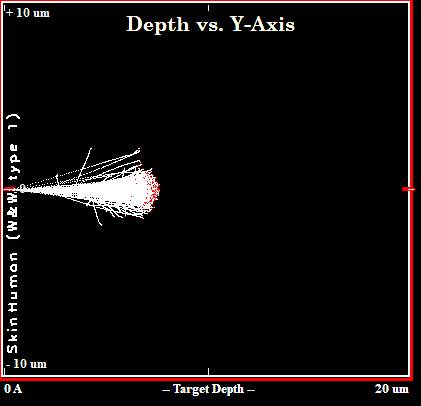
\includegraphics[width=\textwidth]{dati/boro_94/alfa_boro_94/alfa_boro_94.png}
                        \caption{$\alpha$ ($E_{\alpha}$ = 1.47 MeV)}
                        \label{fig:alpha_boro_94}
                    \end{subfigure}\hfill
                    \begin{subfigure}{0.33\textwidth}  
                        \centering
                        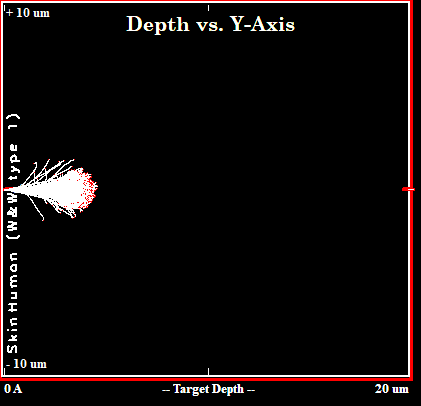
\includegraphics[width=\textwidth]{dati/boro_94/litio_boro_94/litio_boro_94.png}
                        \caption{Litio ($E_{Li}$ = 0.84 MeV)}
                        \label{fig:litio_boro_94}
                    \end{subfigure}\hfill
                \end{figure}
                \item Litio
                \begin{figure}[H]
                    \centering
                    \begin{subfigure}{0.33\textwidth}  
                        \centering
                        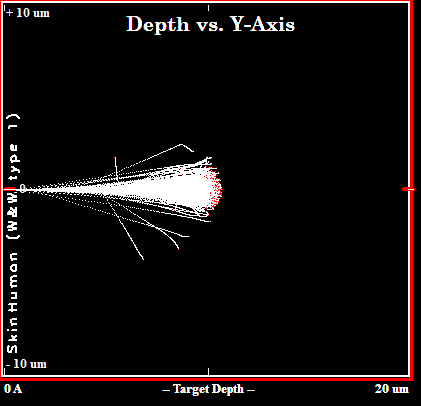
\includegraphics[width=\textwidth]{dati/litio/alfa_litio/alfa_litio.png}
                        \caption{$\alpha$ ($E_{\alpha}$ = 2.05 MeV)}
                        \label{fig:alpha_litio}
                    \end{subfigure}\hfill
                    \begin{subfigure}{0.33\textwidth}  
                        \centering
                        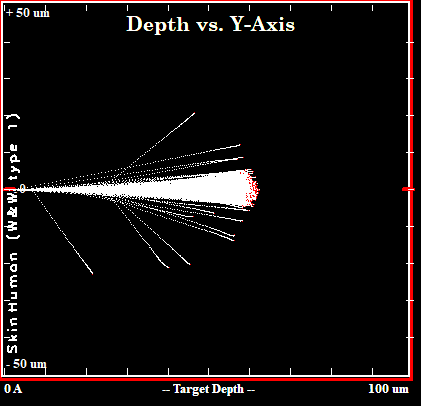
\includegraphics[width=\textwidth]{dati/litio/tritone_litio/tritone_litio.png}
                        \caption{Tritone ($E_{H}$ = 2.73 MeV)}
                        \label{fig:tritone_litio}
                    \end{subfigure}\hfill
                \end{figure}
                \item Azoto
                \begin{figure}[H]
                    \centering
                    \begin{subfigure}{0.33\textwidth}  
                        \centering
                        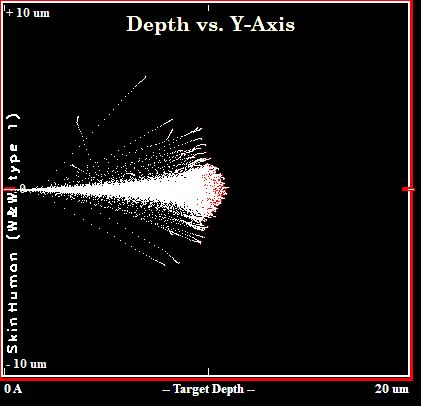
\includegraphics[width=\textwidth]{dati/azoto_non_montecarlo/protone_azoto/protone_azoto.png}
                        \caption{Protoni ($E_{H}$ = 0.584 MeV)}
                        \label{fig:protoni_azoto}
                    \end{subfigure}\hfill
                    \begin{subfigure}{0.33\textwidth}  
                        \centering
                        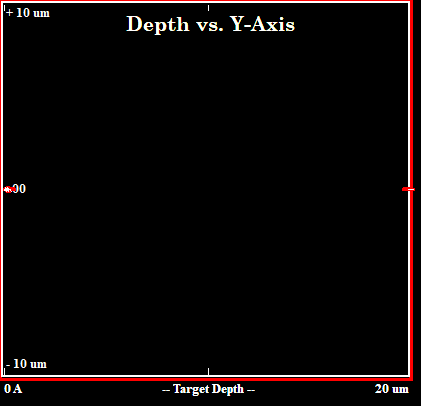
\includegraphics[width=\textwidth]{dati/azoto_non_montecarlo/carbonio_azoto/carbonio_azoto.png}
                        \caption{Carbonio ($E_{C}$ = 0.042 MeV)}
                        \label{fig:carbonio_azoto}
                    \end{subfigure}\hfill
                \end{figure}
            \end{itemize}    
            
            \textbf{Decadimento casuale all'interno della cellula}
            \begin{itemize}
                \item Boro: decadimento con branching ratio 6\%
                \begin{figure}[H]
                    \centering
                    \begin{subfigure}{0.33\textwidth}  
                        \centering
                        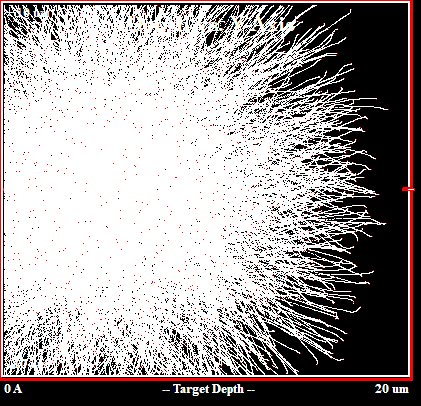
\includegraphics[width=\textwidth]{dati/boro_6_montecarlo/alfa_boro_6_montecarlo/alfa_boro_6_montecarlo.png}
                        \caption{$\alpha$ ($E_{\alpha}$ = 1.78 MeV)}
                        \label{fig:alpha_boro_6_montecarlo}
                    \end{subfigure}\hfill
                    \begin{subfigure}{0.33\textwidth}  
                        \centering
                        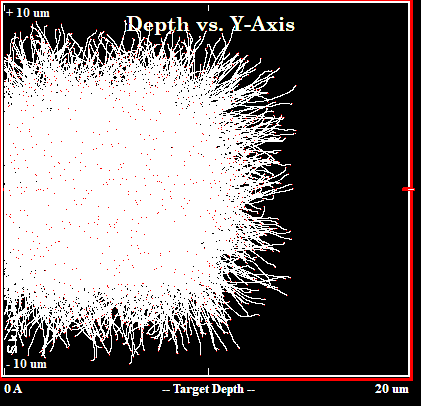
\includegraphics[width=\textwidth]{dati/boro_6_montecarlo/litio_boro_6_montecarlo/litio_boro_6_montecarlo.png}
                        \caption{Litio ($E_{Li}$ = 1.01 MeV)}
                        \label{fig:litio_boro_6_montecarlo}
                    \end{subfigure}\hfill
                \end{figure}
                \item Boro: decadimento con branching ratio 94\%
                \begin{figure}[H]
                    \centering
                    \begin{subfigure}{0.33\textwidth}  
                        \centering
                        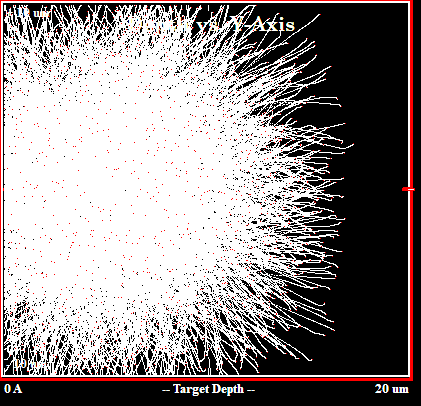
\includegraphics[width=\textwidth]{dati/boro_94_montecarlo/alfa_boro_94_montecarlo/alfa_boro_94_montecarlo.png}
                        \caption{$\alpha$ ($E_{\alpha}$ = 1.47 MeV)}
                        \label{fig:alpha_boro_94_montecarlo}
                    \end{subfigure}\hfill
                    \begin{subfigure}{0.33\textwidth}
                        \centering
                        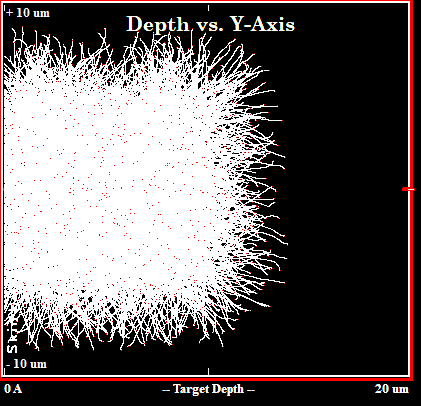
\includegraphics[width=\textwidth]{dati/boro_94_montecarlo/litio_boro_94_montecarlo/litio_boro_94_montecarlo.png}
                        \caption{Litio ($E_{Li}$ = 0.84 MeV)}
                        \label{fig:litio_boro_94_montecarlo}
                    \end{subfigure}\hfill
                \end{figure}
                \item Litio
                \begin{figure}[H]
                    \centering
                    \begin{subfigure}{0.33\textwidth}  
                        \centering
                        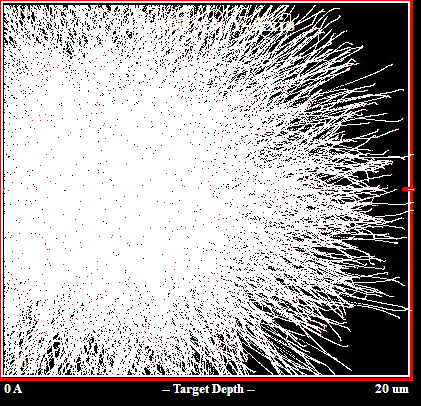
\includegraphics[width=\textwidth]{dati/litio_montecarlo/alfa_litio_montecarlo/alfa_litio_montecarlo.png}
                        \caption{$\alpha$ ($E_{\alpha}$ = 2.05 MeV)}
                        \label{fig:alpha_litio_montecarlo}
                    \end{subfigure}\hfill
                    \begin{subfigure}{0.33\textwidth}  
                        \centering
                        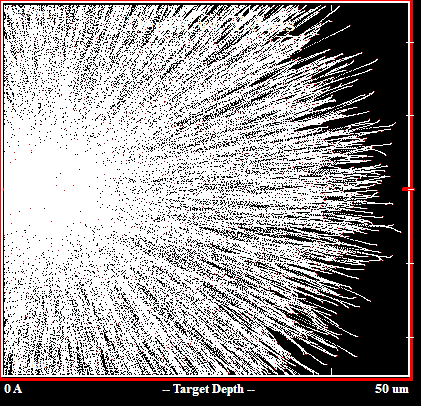
\includegraphics[width=\textwidth]{dati/litio_montecarlo/tritone_litio_montecarlo/tritone_litio_montecarlo.png}
                        \caption{Tritone ($E_{H}$ = 2.73 MeV)}
                        \label{fig:tritone_litio_montecarlo}
                    \end{subfigure}\hfill
                \end{figure}
                \item Azoto
                \begin{figure}[H]
                    \centering
                    \begin{subfigure}{0.33\textwidth}  
                        \centering
                        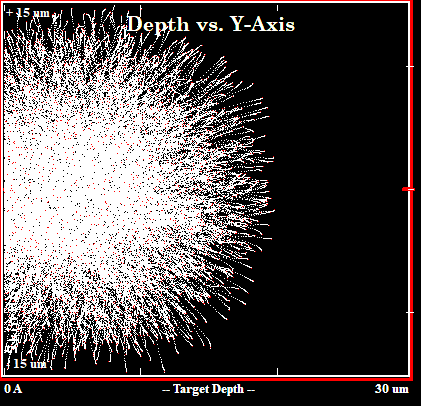
\includegraphics[width=\textwidth]{dati/azoto_montecarlo/protone_azoto_montecarlo/protone_azoto_montecarlo.png}
                        \caption{Protoni ($E_{H}$ = 0.584 MeV)}
                        \label{fig:protoni_azoto_montecarlo}
                    \end{subfigure}\hfill
                    \begin{subfigure}{0.33\textwidth}  
                        \centering
                        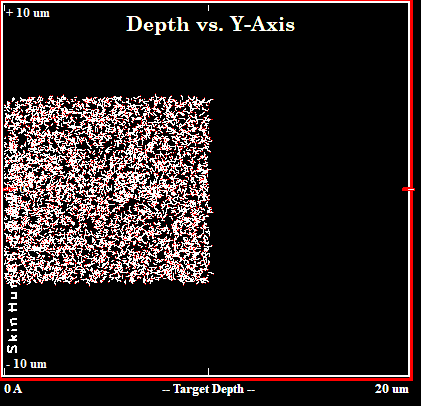
\includegraphics[width=\textwidth]{dati/azoto_montecarlo/carbonio_azoto_montecarlo/carbonio_azoto_montecarlo.png}
                        \caption{Carbonio ($E_{C}$ = 0.042 MeV)}
                        \label{fig:carbonio_azoto_montecarlo}
                    \end{subfigure}\hfill
                \end{figure}
            \end{itemize}

        \subsection{Tabelle Risultati Fit}
            Usando come tessuto la pelle umana SRIM restituisce una densità di 1.09 \unit{\gram \centi\meter^{-3}}. 
            Essendo le cellule modellate come dei cubi di lato 10 \unit{\micro\meter} si ottiene un volume di $\num{1e-09} \unit{cm^3}$.
            Quindi la massa della cellula è di $\num{1e-12} \unit{\kilo\gram}$.
            Qui sotto troviamo le tabelle con le dosi assorbite dalla cellula e da quelle limitrofe nei vari casi studiati.
            \begin{table}[H]
                \centering
                \resizebox{\textwidth}{!}{%
                \begin{tabular}{
                    ll |  cc | cc |
                }
                    \toprule
                    & & \multicolumn{2}{c|}{Cellula sorgente} & \multicolumn{2}{c|}{Cellula limitrofa} \\
                    \cmidrule(lr){3-4}
                    \cmidrule(lr){5-6}
                    & & Energia [\unit{\joule}] & Dose [\unit{\gray}] & Energia [\unit{\joule}] & Dose [\unit{\gray}] \\
                    \midrule
                    \multirow{2}{*}{Boro 6\%} & $\alpha$ & \num{2.83e-13} & \num{2.60e-1} & 0 & 0 \\
                    & $Litio$ & \num{1.57e-13} & \num{1.44e-1} & 0 & 0 \\
                    \midrule
                    \multirow{2}{*}{Boro 94\%} & $\alpha$ & \num{2.34e-13} & \num{2.14e-1} & 0 & 0 \\
                    & $Litio$ & \num{1.30e-13} & \num{1.19e-1} & 0 & 0 \\
                    \midrule
                    \multirow{2}{*}{Litio} & $\alpha$ & \num{3.25e-13} & \num{2.98e-1} & \num{1.63e-15} & \num{1.5e-3} \\
                    & $Tritone$ & \num{4.81e-14} & \num{4.41e-2} & \num{5.23e-14} & \num{4.79e-2} \\
                    \midrule
                    \multirow{2}{*}{Azoto} & $Protone$ & \num{9.19e-14} & \num{8.43e-2} & \num{1.33e-15} & \num{1.22e-3} \\
                    & $Carbonio$ & \num{3.53e-15} & \num{3.24e-3} & 0 & 0 \\
                    \bottomrule
                \end{tabular}%
                }
                \caption{Tabella energia e dose assorbita dalla cellula sorgente e da quella limitrofa nel caso di decadimento sulla superficie}
                \label{tab:dati_prima_misura}
            \end{table}

            Per la seconda parte dell'esperienza si sono presi i dati ottenuti dalle precedenti simulazioni, ma invece di considerare il punto 0 come sulla superficie del cubo si è considerato in centro a questo.
            Quindi i primi 5 \unit{\micro\meter} sono della cellula sorgente e i successivi 10 \unit{\micro\meter} si considerano della cellula limitrofa.
            In questo modo si riesce a calcolare la dose assorbita dalle due cellule nel caso di un decadimento al centro della cellula sorgente.
            \begin{table}[H]
                \centering
                \resizebox{\textwidth}{!}{%
                \begin{tabular}{
                    ll | cc | cc |
                }
                    \toprule
                    & & \multicolumn{2}{c|}{Cellula sorgente} & \multicolumn{2}{c|}{Cellula limitrofa} \\
                    \cmidrule(lr){3-4}
                    \cmidrule(lr){5-6}
                    & & Energia [\unit{\joule}] & Dose [\unit{\gray}] & Energia [\unit{\joule}] & Dose [\unit{\gray}] \\
                    \midrule
                    \multirow{2}{*}{Boro 6\%} & $\alpha$ & \num{1.76e-13} & \num{3.22e-1} & \num{1.07e-13} & \num{9.85e-2} \\
                    & $Litio$ & \num{1.57e-13} & \num{2.88e-1} & 0 & 0 \\
                    \midrule
                    \multirow{2}{*}{Boro 94\%} & $\alpha$ & \num{1.88e-13} & \num{3.38e-1} & \num{4.54e-14} & \num{4.17e-2} \\
                    & $Litio$ & \num{1.30e-13} & \num{2.39e-1} & 0 & 0 \\
                    \midrule
                    \multirow{2}{*}{Litio} & $\alpha$ & \num{1.60e-13} & \num{2.94e-1} & \num{1.66e-13} & \num{1.52e-1} \\
                    & $Tritone$ & \num{2.36e-14} & \num{4.33e-2} & \num{5.00e-14} & \num{4.59e-2} \\
                    \midrule
                    \multirow{2}{*}{Azoto} & $Protone$ & \num{3.51e-14} & \num{6.44e-2} & \num{5.81e-14} & \num{5.33e-3} \\
                    & $Carbonio$ & \num{3.53e-15} & \num{6.49e-3} & 0 & 0 \\
                    \bottomrule
                \end{tabular}%
                }
                \caption{Tabella energia e dose assorbita dalla cellula sorgente e da quella limitrofa nel caso di decadimento al centro della cellula}
                \label{tab:dati_seconda_misura}
            \end{table}

            Anche per l'ultimo punto abbiamo calcolato la dose assorbita dalla cellula sorgente e da quella limitrofa.
            \begin{table}[H]
                \centering
                \resizebox{\textwidth}{!}{%
                \begin{tabular}{
                    ll | cc | cc |
                }
                    \toprule
                    & & \multicolumn{2}{c|}{Cellula sorgente} & \multicolumn{2}{c|}{Cellula limitrofa} \\
                    \cmidrule(lr){3-4}
                    \cmidrule(lr){5-6}
                    & & Energia [\unit{\joule}] & Dose [\unit{\gray}] & Energia [\unit{\joule}] & Dose [\unit{\gray}] \\
                    \midrule
                    \multirow{2}{*}{Boro 6\%} & $\alpha$ & \num{1.11e-13} & \num{2.04e-1} & \num{1.40e-13} & \num{1.28e-1} \\
                    & $Litio$ & \num{7.18e-14} & \num{1.32e-1} & \num{7.93e-14} & \num{7.27e-2} \\
                    \midrule
                    \multirow{2}{*}{Boro 94\%} & $\alpha$ & \num{9.72e-14} & \num{1.78e-1} & \num{1.17e-13} & \num{1.08e-1} \\
                    & $Litio$ & \num{6.19e-14} & \num{1.14e-1} & \num{6.35e-14} & \num{5.83e-2} \\
                    \midrule
                    \multirow{2}{*}{Litio} & $\alpha$ & \num{1.21e-13} & \num{2.22e-1} & \num{1.62e-13} & \num{1.49e-1} \\
                    & $Tritone$ & \num{5.07e-14} & \num{9.29e-2} & \num{8.56e-14} & \num{7.86e-2} \\
                    \midrule
                    \multirow{2}{*}{Azoto} & $Protone$ & \num{3.32e-14} & \num{6.09e-2} & \num{4.47e-14} & \num{4.10e-2} \\
                    & $Carbonio$ & \num{1.79e-15} & \num{3.28e-3} & \num{1.74e-15} & \num{1.60e-3} \\
                    \bottomrule
                \end{tabular}%
                }
                \caption{Tabella energia e dose assorbita dalla cellula sorgente e da quella limitrofa nel caso di decadimento al centro della cellula}
                \label{tab:dati_terza_misura}
            \end{table}
    % -------------------------------------------------------------------
    \section{Conclusioni}
        
\end{document}